\begin{figure}[H]
	\centering
	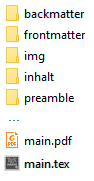
\includegraphics[scale=1]{ordner}
	\caption{Beispiel für Datenorganisation}
\end{figure}

Je nach Editor und Kompilierungseinstellungen
kann es vorkommen, dass ein \texttt{build} Ordner
erstellt wird, in dem die temporären Dateien 
(\texttt{.aux, .log}, usw.) sich befinden.
So sieht das Arbeitsverzeichnis sauberer aus!
